\begin{figure}[H]
    \centering
    \begin{subfigure}[t]{0.48\textwidth}
        \centering
        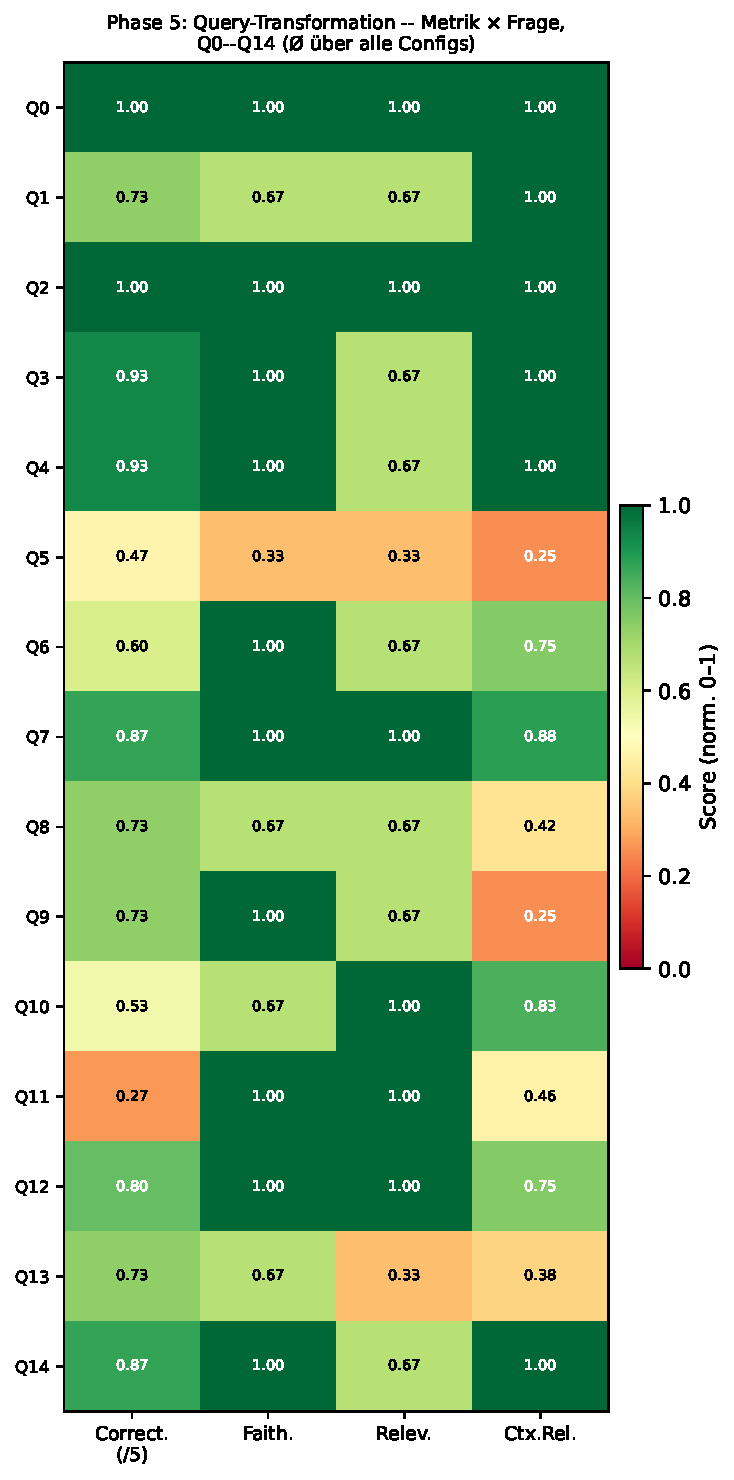
\includegraphics[width=\textwidth]{img/results/phase5_metrics_a.pdf}
        \caption{Q0--Q14}
        \label{fig:phase5_metrics_a}
    \end{subfigure}
    \hfill
    \begin{subfigure}[t]{0.48\textwidth}
        \centering
        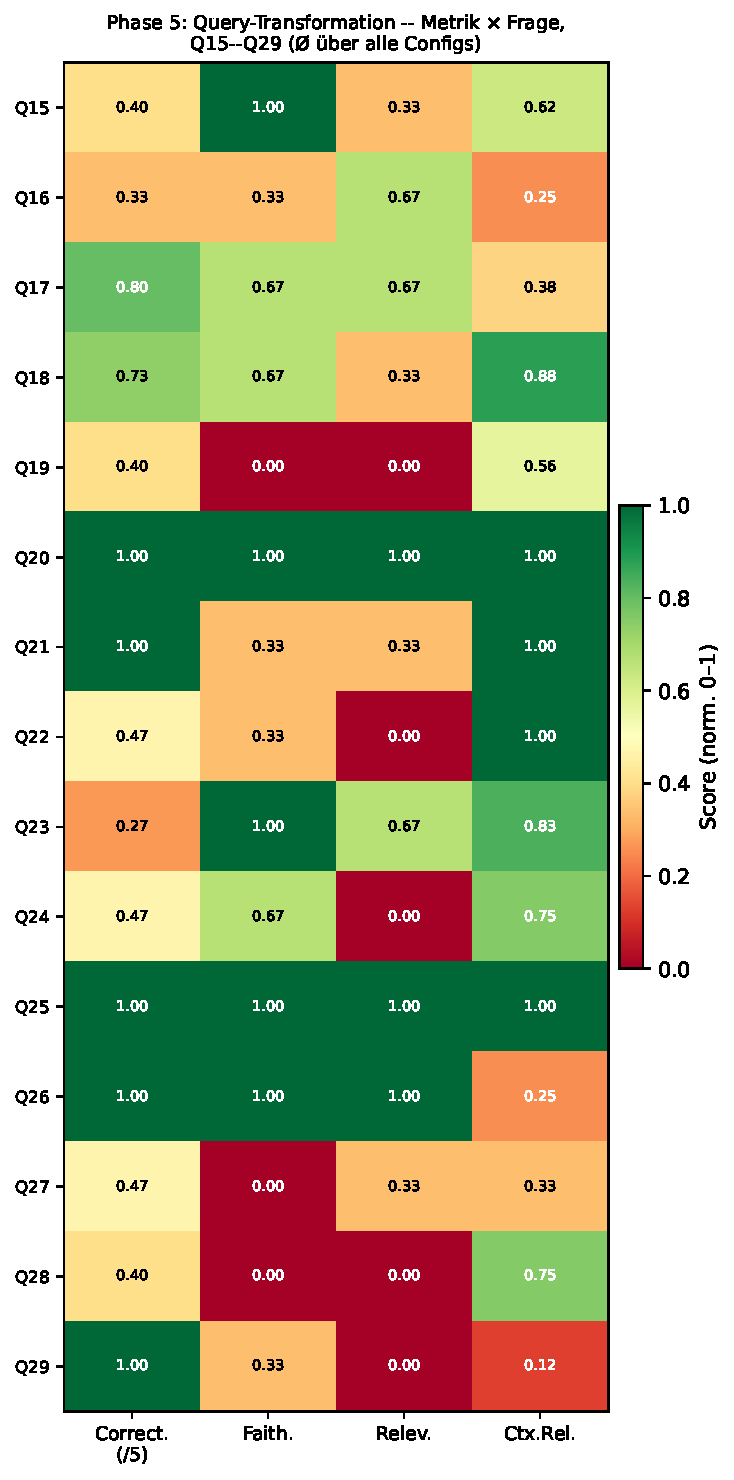
\includegraphics[width=\textwidth]{img/results/phase5_metrics_b.pdf}
        \caption{Q15--Q29}
        \label{fig:phase5_metrics_b}
    \end{subfigure}
    \caption{Phase 5: Query-Transformation -- Metrik × Frage (Ø über alle Konfigurationen)}
    \label{fig:phase5_metrics}
\end{figure}
